% !TEX root = task-4-6.tex
% Editable task bank. Append new BankTask blocks at the end of the document.
\documentclass[12pt,a4paper]{article}
\usepackage{physics-textbook}
\usepackage{graphicx,needspace}
\usetikzlibrary{decorations.pathmorphing}
\newif\ifShowSolutions
\ifdefined\TutorEdition
  \ShowSolutionstrue
\else
  \ShowSolutionsfalse % Change to \ShowSolutionstrue to display solutions.
\fi
\newcounter{banktask}
\newsavebox{\BankTaskBox}
\newcommand{\BankTaskContent}[3]{%
  \noindent\textbf{\thebanktask.}\quad #2\par
  \ifShowSolutions
    \Needspace{50mm}% Keep the solution heading with its opening text or diagram.
    #3\par
    \ifdefined\TutorEdition
      \ifcsname TutorSource#1\endcsname
        \nopagebreak\smallskip{\small\csname TutorSource#1\endcsname\par}%
      \fi
    \fi
  \fi
}
\newcommand{\BankTask}[3]{%
  \refstepcounter{banktask}\par\medskip
  \sbox{\BankTaskBox}{\begin{minipage}{\linewidth}%
    \BankTaskContent{#1}{#2}{#3}\end{minipage}}%
  \ifdim\dimexpr\ht\BankTaskBox+\dp\BankTaskBox\relax>\dimexpr\textheight-20mm\relax
    \Needspace{35mm}\BankTaskContent{#1}{#2}{#3}%
  \else
    \Needspace{\dimexpr\ht\BankTaskBox+\dp\BankTaskBox\relax}%
    \noindent\usebox{\BankTaskBox}\par
  \fi
  \medskip
}
\begin{document}
\BookSubsection{4.6}{Тонкие линзы. Построение изображений}


% Source sdamgia-39952: https://phys-ege.sdamgia.ru/problem?id=39952
\BankTask{sdamgia-39952}{
Небольшой предмет расположен на главной оптической оси тонкой собирающей линзы с фокусным расстоянием $15\,\text{см}$. Расстояние от линзы до действительного изображения предмета составляет $30\,\text{см}$. Определите расстояние от линзы до предмета.
}{
\smallskip\noindent\textbf{Решение}\par
Поскольку линза собирающая и расстояние между линзой и предметом больше фокусного расстояния, заключаем, что линза будет давать действительное изображение, располагающееся за линзой. Согласно формуле тонкой линзы, расстояния от линзы до предмета d и до изображения f связаны с фокусным расстоянием соотношением: $\frac{1}{F} = \frac{1}{d} + \frac{1}{f} .$ Отсюда искомое расстояние равно: 

\[d = \frac{fF}{f - F} = \frac{30\,\text{см} \cdot 15\,\text{см}}{30\,\text{см} - 15\,\text{см}} = 30\,\text{см}.\]

Ответ: $30$.
}

% Source sdamgia-1726: https://phys-ege.sdamgia.ru/problem?id=1726
\BankTask{sdamgia-1726}{
На рисунке показан ход лучей от точечного источника света А через тонкую линзу.

\begin{center}\begin{tikzpicture}[x=.38cm,y=.38cm,>=stealth]
\draw[task grid,xstep=.38cm,ystep=.38cm] (0,0) grid (28,10);
\draw[thick] (0,5)--(28,5);
\draw[<->,thick] (14,1)--(14,9);
\draw[<->,thick] (18,8)--(23,8) node[midway,above] {$5\,\text{см}$};
\draw[thick,orange!85!black] (1,7)--(14,7)--(27.75,2.417);
\draw[thick,orange!85!black] (1,7)--(27.45,2.931);
\draw[->,thick,orange!85!black] (7.1,7)--(8.1,7)
 (22.2,4.267)--(23.15,3.95) (19.25,4.192)--(20.25,4.038);
\draw[->,thick,orange!85!black] (26.75,2.75)--(27.75,2.417) (26.45,3.085)--(27.45,2.931);
\fill[orange!85!black] (1,7) circle (.16);
\node[above right] at (1,7) {$A$};
\end{tikzpicture}\end{center}

Какова оптическая сила линзы в диоптриях? Округлите до целых.
}{
\smallskip\noindent\textbf{Решение}\par
Оптическая сила линзы обратно пропорциональна фокусному расстоянию: $D= \frac{1}{F} .$ Определим фокусное расстояние. Луч, параллельный главной оптической оси, после преломления в тонкой линзе пройдет через главный фокус. Из рисунка видно, что такой луч пересекает главную оптическую ось на расстоянии $6$ клеток от линзы. Поскольку масштаб рисунка одна сторона клетки  — $1\,\text{см}$, получаем, что $F=0{,}06\,\text{м}.$ Следовательно, оптическая сила линзы равна приблизительно $D= \frac{1}{0{,}06\,\text{м}} \approx 17\,\text{дптр}.$

Ответ: $17$.
}

% Source sdamgia-19879: https://phys-ege.sdamgia.ru/problem?id=19879
\BankTask{sdamgia-19879}{
\begin{center}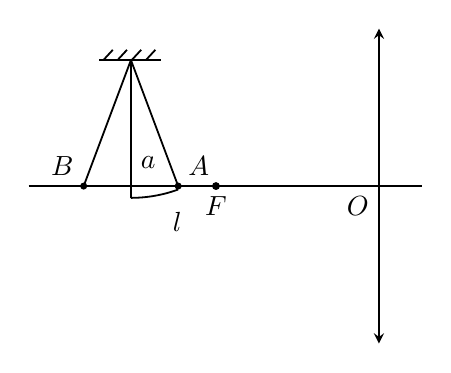
\begin{tikzpicture}[>=stealth,line width=.65pt]\draw(-4,0)--(1,0);\draw[<->](.45,-2)--(.45,2);\draw(-2.7,1.6)--(-3.3,0) (-2.7,1.6)--(-2.1,0) (-2.7,1.6)--(-2.7,-.15);\draw (-2.7,-.15) arc (-90:-70:1.75);\draw(-3.1,1.6)--(-2.32,1.6);\foreach \x in {-3.05,-2.87,...,-2.33} {\draw (\x,1.6)--++(.12,.13);}\fill(-3.3,0)circle(.045)node[above left]{$B$};\fill(-2.1,0)circle(.045)node[above right]{$A$};\fill(-1.62,0)circle(.05)node[below]{$F$};\node[below left]at(.45,0){$O$};\node at(-2.48,.3){$a$};\node at(-2.11,-.45){$l$};\end{tikzpicture}\end{center}

Шарик подвешен на нити и совершает колебания. Его крайние точки, А и B, лежат на оптической оси собирающей линзы силой D  =  $50\,\text{дптр}$. Проекция точки равновесия шарика находится на расстоянии $\sqrt{5}$ см от первого фокуса линзы. Расстояние от нее до крайних точек равно $1\,\text{см}$. Найдите расстояние между изображениями крайних точек A и B в собирающей линзе.
}{
\smallskip\noindent\textbf{Решение}\par
\begin{center}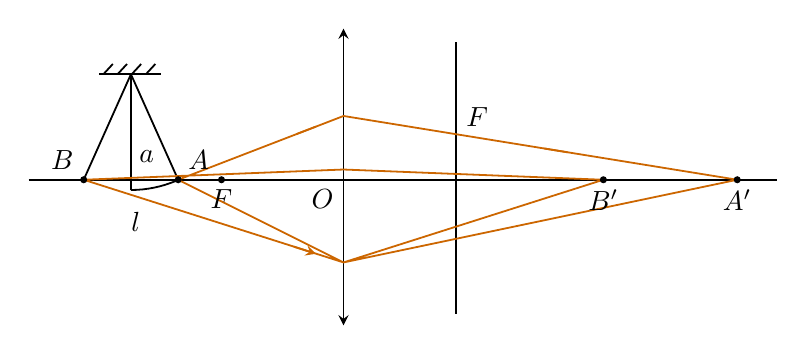
\begin{tikzpicture}[>=stealth,line width=.65pt]\draw(-4,0)--(5.5,0);\draw[<->](0,-1.85)--(0,1.92);\draw(1.43,-1.7)--(1.43,1.75);\draw(-2.7,1.34)--(-3.3,0) (-2.7,1.34)--(-2.1,0) (-2.7,1.34)--(-2.7,-.13);\draw(-2.7,-.13)arc(-90:-67:1.47);\draw(-3.1,1.34)--(-2.32,1.34);\foreach \x in {-3.05,-2.87,...,-2.33} {\draw (\x,1.34)--++(.12,.13);}\draw[orange!80!black](-2.1,0)--(0,.81)--(5,0) (-2.1,0)--(0,-1.05)--(5,0) (-3.3,0)--(0,.13)--(3.3,0) (-3.3,0)--(0,-1.05)--(3.3,0);\draw[->,orange!80!black](-.6,.579)--(-.35,.675) (2.55,.397)--(2.85,.348) (-.63,-.85)--(-.35,-.94);\fill(-3.3,0)circle(.045)node[above left]{$B$};\fill(-2.1,0)circle(.045)node[above right]{$A$};\fill(3.3,0)circle(.045)node[below]{$B^{\prime}$};\fill(5,0)circle(.045)node[below]{$A^{\prime}$};\fill(-1.55,0)circle(.045)node[below]{$F$};\node[above right]at(1.43,.55){$F$};\node[below left]at(0,0){$O$};\node at(-2.5,.3){$a$};\node at(-2.64,-.54){$l$};\end{tikzpicture}\end{center}

Запишем уравнения для тонкой линзы: $\frac{1}{F} = \frac{1}{OB} + \frac{1}{OB'} ;$ $\frac{1}{F} = \frac{1}{OA} + \frac{1}{OA'} .$ По определению $D= \frac{1}{F} ,$ следовательно, $F= \frac{1}{D} =2 \,\text{см}.$ Откуда

$OA=F + l - A=2 + \sqrt{5} - 1=1 + \sqrt{5} \,\text{см},$ 
$OB=F + l + A=3 + \sqrt{5} \,\text{см}.$

Тогда 

$\frac{1}{OB'} = \frac{1}{F} - \frac{1}{OB} =50 - \frac{1}{( 3 + \sqrt{5} ) \cdot 0{,}01} =25 ( \sqrt{5} - 1 ) ;$
$OB'= \frac{1}{25 ( \sqrt{5} - 1 )} = \frac{\sqrt{5} + 1}{100} \,\text{м};$
$\frac{1}{OA'} = \frac{1}{F} - \frac{1}{OA} =50 - \frac{1}{( 1 + \sqrt{5} ) \cdot 0{,}01} =25 ( 3 - \sqrt{5} ) ;$
$OA'= \frac{1}{25 ( 3 - \sqrt{5} )} = \frac{3 + \sqrt{5}}{100} \,\text{м};$
$|OA' - OB'|=| \frac{\sqrt{5} + 1 - 3 - \sqrt{5}}{100} |= \frac{1}{50} \,\text{м} = 2\,\text{см}.$

Ответ: $|OA' - OB'|=2\,\text{см}.$
}

% Source sdamgia-29760: https://phys-ege.sdamgia.ru/problem?id=29760
\BankTask{sdamgia-29760}{
Рассеивающая линза с фокусным расстоянием $F_1=10$ см расположена перед собирающей линзой с фокусными расстоянием $F_2=15$ см. Лучи, идущие от точечного источника света, расположенного на расстоянии $d=10$ см от pacceивающей линзы, пройдя систему образовали пучок лучей, параллельный главной оптической оси. Найдите расстояние между линзами.
}{
\smallskip\noindent\textbf{Решение}\par
$1$.  Найдем расстояние от рассеивающей линзы до изображения точечного источника света по формуле тонкой линзы 

\[\frac{1}{d} - \frac{1}{f} = - \frac{1}{F_1} ,\]

 откуда 

\[f= \frac{d F_1}{d + F_1} = \frac{10 \cdot 10}{10 + 10} =5 \,\text{см}.\]

 Это мнимое изображение находится перед рассеивающей линзой. 
$2$.  Учитывая, что данная точка является источником для собирающей линзы, а лучи после прохождения через нее параллельны, делаем вывод, что эта точка находится в фокусе собирающей линзы, то есть на расстоянии $15\,\text{см}$.
$3$.  Тогда расстояние между линзами равно $x=F_2 - f=15 - 5=10 \,\text{см}.$ 

Ответ: $10\,\text{см}$.
}

% Source sdamgia-50813: https://phys-ege.sdamgia.ru/problem?id=50813
\BankTask{sdamgia-50813}{
Линза, фокусное расстояние которой $30\,\text{см}$, даёт на экране резкое изображение предмета c пятикратным увеличением. Экран пододвинули к линзе вдоль её главной оптической оси. Затем при неизменном положении линзы передвинули предмет на $3\,\text{см}$ так, чтобы изображение снова стало резким. На какое расстояние сдвинули экран относительно его первоначального положения? Сделайте рисунок построения изображений в линзе с указанием хода лучей.
}{
\smallskip\noindent\textbf{Решение}\par
Построим изображение предмета в собирающей линзе в первом случае:


\begin{center}\begin{tikzpicture}[>=stealth,line width=.65pt]\draw (-2.1,0)--(7.95,0);\draw[<->](0,-2.55)--(0,2.55);\draw[cyan!50,line width=2.5pt](7.5,-2.48)--(7.5,2.46);\node[below]at(7.5,-2.5){Экран};\draw[->,orange!80!black](-1.5,0)node[below left]{$B$}--(-1.5,.35)node[above left]{$A$};\draw[->,red!70!black](7.5,0)node[below left]{$C$}--(7.5,-1.75)node[below left]{$D$};\draw[green!55!black](-1.5,.35)--(0,.35)--(7.5,-1.75) (-1.5,.35)--(7.5,-1.75);\draw[->,green!55!black](-1,.35)--(-.64,.35);\draw[->,green!55!black](1.8,{-.35*1.8/1.5})--(2.14,{-.35*2.14/1.5});\draw[->,green!55!black](2.65,{.35-.28*2.65})--(3,{.35-.28*3});\fill(-1.25,0)circle(.026)node[below right]{$F$};\fill(1.25,0)circle(.026)node[above]{$F$};\node[below left]at(0,0){$O$};\draw[thin](-1.5,.38)--(-1.5,2.15);\draw[<->](-1.5,2.1)--(0,2.1)node[midway,above]{$d_1$};\draw[<->](0,2.1)--(7.5,2.1)node[midway,above]{$f_1$};\end{tikzpicture}\end{center}


Используем формулы тонкой линзы $\frac{1}{d_1} + \frac{1}{f_1} = \frac{1}{F}$ и увеличения, даваемого собирающей линзой, $\Gamma = \frac{f_1}{d_1} .$ Из них находим расстояние от предмета до линзы и от изображения до линзы: $d_1 = 1{,}2F,$ $f_1 = 6F.$
Построим изображение предмета в собирающей линзе во втором случае:


\begin{center}\begin{tikzpicture}[>=stealth,line width=.65pt]\draw (-2.1,0)--(7.95,0);\draw[<->](0,-2.55)--(0,2.55);\draw[cyan!50,line width=2.5pt](5.4167,-2.48)--(5.4167,2.46);\node[below]at(5.4167,-2.5){Экран};\draw[->,orange!80!black](-1.625,0)node[below left]{$B$}--(-1.625,.35)node[above left]{$A$};\draw[->,red!70!black](5.4167,0)node[below left]{$C_1$}--(5.4167,-1.166673846153846)node[below left]{$D_1$};\draw[green!55!black](-1.625,.35)--(0,.35)--(5.4167,-1.166673846153846) (-1.625,.35)--(5.4167,-1.166673846153846);\draw[->,green!55!black](-1,.35)--(-.64,.35);\draw[->,green!55!black](1.8,{-.35*1.8/1.625})--(2.14,{-.35*2.14/1.625});\draw[->,green!55!black](2.65,{.35-.28*2.65})--(3,{.35-.28*3});\fill(-1.25,0)circle(.026)node[below right]{$F$};\fill(1.25,0)circle(.026)node[above]{$F$};\node[below left]at(0,0){$O$};\draw[thin](-1.625,.38)--(-1.625,2.15);\draw[<->](-1.625,2.1)--(0,2.1)node[midway,above]{$d_2$};\draw[<->](0,2.1)--(5.4167,2.1)node[midway,above]{$f_2$};\draw[dashed](-1.5,0)--(-1.5,2.15) (7.5,-2.3)--(7.5,2.22);\draw[<->](-1.5,1.68)--(-1.625,1.68)node[midway,left=.24cm]{$\Delta d$};\draw[<->](5.4167,2.1)--(7.5,2.1)node[midway,above]{$x$};\end{tikzpicture}\end{center}


При этом видно, что если по условию расстояние от линзы до экрана уменьшили на величину x, то расстояние от предмета до линзы увеличилось на величину $\Delta d.$ Запишем формулу собирающей линзы для этого случая:

$\frac{1}{d_2} + \frac{1}{f_2} = \frac{1}{F} ,$
$\frac{1}{d_1 + \Delta d} + \frac{1}{f_1 - x} = \frac{1}{F} ,$
$\frac{1}{1{,}2F + \Delta d} + \frac{1}{6F - x} = \frac{1}{F} ,$

откуда находим искомое расстояние:

\[x = \frac{5F \Delta d}{0{,}2F + \Delta d} = \frac{5 \cdot 30 \cdot 3}{0{,}2 \cdot 30 + 3} = 50 \,\text{см}.\]

Ответ: $50\,\text{см}$.
}

% Source sdamgia-7902: https://phys-ege.sdamgia.ru/problem?id=7902
\BankTask{sdamgia-7902}{
\begin{center}\begin{tikzpicture}[>=stealth,line width=.65pt]\draw (-4.65,0)--(3.4,0) (-2,-1.95)--(-2,1.95) (0,-1.95)--(0,1.95);\node[above]at(-2,1.95){Э};\node[above]at(0,1.95){Л};\fill (-4.3,.85)circle(.055)node[above left]{$S$};\draw[thin](-4.3,0)--(-4.3,.85)node[midway,left]{$H$};\node[below]at(-3.1,0){$b$};\fill (-2,-.68)circle(.035)node[left]{$A$};\node[right]at(-2,-.36){$h$};\node[above right]at(-2,0){$F$};\fill (2,0)circle(.045)node[above]{$F$};\end{tikzpicture}\end{center}

На расстоянии b = $40\,\text{см}$ от собирающей линзы с фокусным расстоянием $20\,\text{см}$ находится точечный источник света, расположенный на высоте Н = $5\,\text{см}$ от главной оптической оси. В левой фокальной плоскости линзы расположен тонкий экран с малым отверстием  А, находящемся в плоскости рисунка на расстоянии h = $4\,\text{см}$ от главной оптической оси. Изобразите ход луча SA и определите, на каком расстоянии х от плоскости линзы этот луч  от точечного источника, пройдя через отверстие в экране и линзу, пересечет главную оптическую ось. Дифракцией пренебречь.
}{
\smallskip\noindent\textbf{Решение}\par
\begin{center}\begin{tikzpicture}[>=stealth,line width=.65pt]\draw (-4.65,0)--(7,0) (-2,-2.3)--(-2,1.8) (0,-2.3)--(0,1.8);\node[above]at(-2,1.8){Э};\node[above]at(0,1.8){Л};\draw[thin](-4,0)--(-4,.8)node[midway,left]{$H$} (4,0)--(4,-.8)node[midway,above left]{$H\prime$};\draw[blue!70!black] (-4,.8)--(0,.8)--(6.7,-1.88) (-4,.8)--(6.7,-1.34);\draw[green!45!black] (-4,.8)--(0,-2.08)--(7,.16);\draw[->,blue!70!black](-1,.8)--(-.8,.8) (1.1,.36)--(1.3,.28) (.9,-.18)--(1.1,-.22);\draw[->,green!45!black](1.1,-1.728)--(1.3,-1.664);\fill(-4,.8)circle(.045)node[above left]{$S$};\fill(4,-.8)circle(.045)node[below left]{$S\prime$};\fill(-2,-.64)circle(.04)node[below left]{$A$};\node[above right]at(-2,0){$F$};\node[right]at(-2,-.33){$h$};\node[below]at(-3,0){$b$};\fill(2,0)circle(.045)node[above]{$F$};\end{tikzpicture}\end{center}

Построим изображение источника $S',$ используя свойства тонкой линзы: луч, идущий параллельно оптической оси, после преломления в линзе проходит через ее фокус; луч, идущий через середину линзы, не преломляется. Луч SA после преломления в линзе также пройдет через точку $S'$ (см. рис.).
Теперь вычислим, где он пересекает оптическую ось. Луч преломляется в линзе на расстоянии y от оптической оси. Из подобия треугольников находим, что

\[\frac{H + h}{b - F} = \frac{y - h}{F} \Longleftrightarrow y= \frac{F ( H + h )}{b - F} + h= \frac{bh + HF}{b - F} .\]

Из точки А проведем луч через оптический центр линзы О, который не преломляется. Точка А является побочным фокусом линзы, поэтому этот луч параллелен преломленному лучу.
Из подобия треугольников находим, что

$\frac{h}{F} = \frac{y}{x}$
$x=y \cdot \frac{F}{h} = \frac{F}{h} \cdot \frac{bh + HF}{b - F} = \frac{20}{4} \cdot \frac{4 \cdot 40 + 20 \cdot 5}{40 - 20} =65\,\text{см}$

Ответ: ход луча изображен на рисунке, $x=65\,\text{см}.$
}

% Source sdamgia-26734: https://phys-ege.sdamgia.ru/problem?id=26734
\BankTask{sdamgia-26734}{
Два точечных источника света находятся на главной оптической оси тонкой собирающей линзы на расстоянии L  =  $1\,\text{м}$ друг от друга. Линза находится между ними. Расстояние от линзы до одного из источников x  =  $20\,\text{см}$. Изображения обоих источников получились в одной точке. Найдите оптическую силу линзы. Постройте на отдельных рисунках изображения двух источников в линзе, указав ход лучей.
}{
\smallskip\noindent\textbf{Решение}\par
$1$.  Так как источники находятся с разных сторон от линзы, то для одного из них изображение должно быть действительным, а для другого  — мнимым (см. рис.).
$2$.  Источник, который находится ближе к линзе, дает мнимое изображение.


\begin{center}\begin{tikzpicture}[>=stealth,line width=.65pt]\draw(-4.3,0)--(3.1,0);\draw[<->](0,-2.55)--(0,2.35)node[left]{Л};\draw[orange!80!black] (-3,0)--(2,1.72) (-1.25,0)--(0,1.03)--(2,1.72) (-1.25,-1.03)--(2.25,1.84);\draw[dashed](2,0)--(2,2.18);\fill(-3,0)circle(.045)node[below left]{$S_1^{\prime}$};\fill(-1.25,0)circle(.045)node[below left]{$S_1$};\fill(-2,0)circle(.045)node[below]{$F$};\fill(2,0)circle(.045)node[below]{$F$};\draw[thin](-3,0)--(-3,-2.35) (-1.25,0)--(-1.25,-1.85);\draw[<->](-3,-2.35)--(0,-2.35)node[midway,above]{$f$};\draw[<->](-1.25,-1.8)--(0,-1.8)node[midway,above]{$x$};\draw[->,orange!80!black](1.4,1.515)--(1.7,1.62) (-.75,.412)--(-.5,.618);\end{tikzpicture}\end{center}


 Источник, который находится дальше от линзы, дает действительное изображение.


\begin{center}\begin{tikzpicture}[>=stealth,line width=.65pt]\draw(-3.25,0)--(4,0);\draw[<->](0,-2.55)--(0,2.35)node[left]{Л};\draw[orange!80!black](3.15,0)--(0,1.38)--(-2,0) (3.15,-1.38)--(-2,1);\draw[dashed](-1.25,0)--(-1.25,2.2);\fill(-2,0)circle(.045)node[below left]{$S_2^{\prime}$};\fill(3.15,0)circle(.045)node[below right]{$S_2$};\fill(-1.25,0)circle(.045)node[below]{$F$};\draw[thin](-2,0)--(-2,-2.35) (3.15,0)--(3.15,-2.35);\draw[<->](-2,-2.35)--(0,-2.35)node[midway,above]{$f$};\draw[<->](0,-2.35)--(3.15,-2.35)node[midway,above]{$L-x$};\draw[->,orange!80!black](1.2,.855)--(.9,.986) (-.8,.83)--(-1,.69);\end{tikzpicture}\end{center}


$3$.  Формулы тонкой линзы для двух источников имеют вид:

$\frac{1}{x} - \frac{1}{f} = \frac{1}{F}$ (минус перед f, так как изображение мнимое), ($1$)
$\frac{1}{L - x} + \frac{1}{f} = \frac{1}{F} ,$ ($2$)

 где F  — фокусное расстояние линзы, f  — расстояние от линзы до точки, в которой находятся оба изображения.
$4$.  Решая систему уравнений ($1$)-($2$), получим:

\[F= \frac{2x ( L - x )}{L} .\]

$5$.  Так как оптическая сила линзы $D= \frac{1}{F} ,$ то получим:

\[D= \frac{L}{2x ( L - x )} = \frac{1}{2 \cdot 0{,}2 ( 1 - 0{,}2 )} =3{,}125 \,\text{дптр}.\]

Ответ: D  =  $3{,}125\,\text{дптр}$.
}

% Source sdamgia-50816: https://phys-ege.sdamgia.ru/problem?id=50816
\BankTask{sdamgia-50816}{
\begin{center}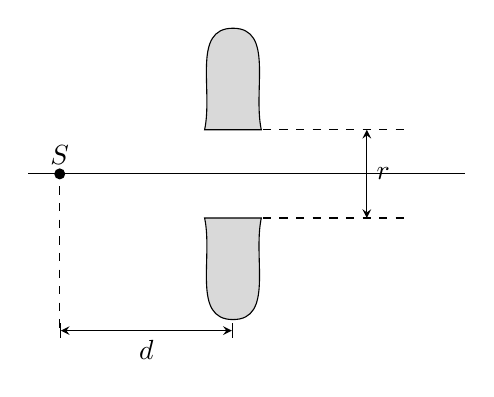
\begin{tikzpicture}[>=stealth]

\draw (-2.6,0)--(2.95,0);\fill (-2.2,0)circle(.07)node[above]{$S$};
\draw[fill=gray!30] (-.36,.56) to[out=78,in=180] (0,1.85) to[out=0,in=102] (.36,.56)--cycle;
\draw[fill=gray!30] (-.36,-.56) to[out=-78,in=180] (0,-1.85) to[out=0,in=-102] (.36,-.56)--cycle;
\draw[dashed](.38,.56)--(2.24,.56) (.38,-.56)--(2.24,-.56);
\draw[<->](1.7,-.56)--(1.7,.56) node[midway,right]{$r$};
\draw[|<->|](-2.2,-1.99)--(0,-1.99)node[midway,below]{$d$};\draw[dashed](-2.2,-.16)--(-2.2,-1.99);
\end{tikzpicture}\end{center}
Точечный источник света находится на главной оптической оси тонкой собирающей линзы. Линзу разрезали на две половины, которые раздвинули на расстояние r  =  $2\,\text{мм}$ (см. рис.). Сделайте рисунок с указанием хода лучей через данную систему. Найдите расстояние от точечного источника света до линзы, если расстояние между действительными изображениями источника l  =  $6\,\text{мм}$. Фокусное расстояние линзы F  =  $40\,\text{см}$.
}{
\smallskip\noindent\textbf{Решение}\par
После того, как линзу разрезали пополам и раздвинули, получилась система из двух линз, у каждой из которой главная оптическая ось поднялась на величину $\frac{r}{2} .$ Построим изображение источника тока через каждую из линз:

\begin{center}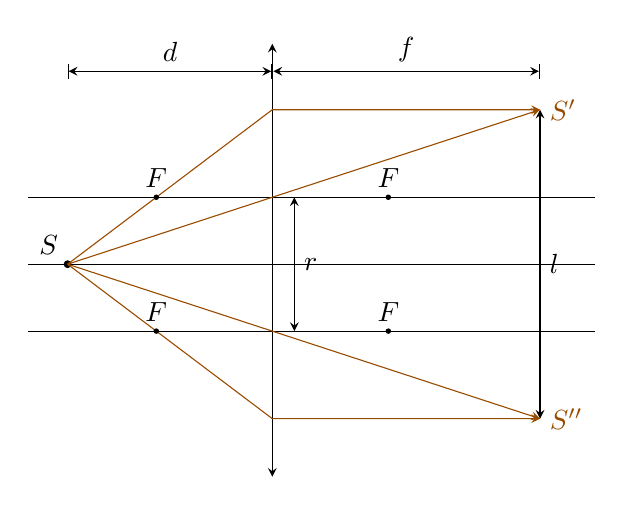
\begin{tikzpicture}[>=stealth]

\draw(-3.1,0)--(4.1,0) (-3.1,.85)--(4.1,.85) (-3.1,-.85)--(4.1,-.85);
\draw[<->](0,-2.7)--(0,2.8);\fill(-2.6,0)circle(.05)node[above left]{$S$};
\draw[orange!60!black,->](-2.6,0)--(0,1.962)--(3.4,1.962)node[right]{$S'$};
\draw[orange!60!black,->](-2.6,0)--(3.4,1.962);
\draw[orange!60!black,->](-2.6,0)--(0,-1.962)--(3.4,-1.962)node[right]{$S''$};
\draw[orange!60!black,->](-2.6,0)--(3.4,-1.962);
\foreach \y in {-.85,.85}{\fill(-1.4733,\y)circle(.035)node[above]{$F$} (1.4733,\y)circle(.035)node[above]{$F$};}
\draw[<->](.28,-.85)--(.28,.85)node[midway,right]{$r$};
\draw[<->](3.4,-1.962)--(3.4,1.962)node[midway,right]{$l$};
\draw[|<->|](-2.6,2.45)--(0,2.45)node[midway,above]{$d$};
\draw[|<->|](0,2.45)--(3.4,2.45)node[midway,above]{$f$};
\end{tikzpicture}\end{center}


\begin{center}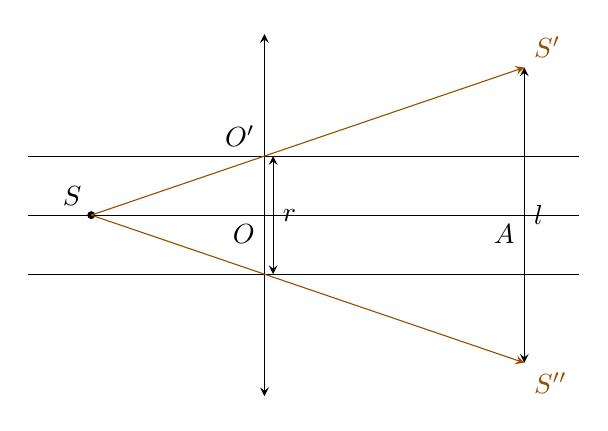
\begin{tikzpicture}[>=stealth]

\draw (-3,0)--(4,0) (-3,.75)--(4,.75) (-3,-.75)--(4,-.75);\draw[<->](0,-2.3)--(0,2.3);
\fill(-2.2,0)circle(.05)node[above left]{$S$};\node[below left]at(0,0){$O$};\node[above left]at(0,.75){$O'$};
\draw[orange!60!black,->](-2.2,0)--(3.3,1.875)node[above right]{$S'$};
\draw[orange!60!black,->](-2.2,0)--(3.3,-1.875)node[below right]{$S''$};
\draw[<->](3.3,-1.875)--(3.3,1.875)node[midway,right]{$l$};\node[below left]at(3.3,0){$A$};
\draw[<->](.11,-.75)--(.11,.75)node[midway,right]{$r$};
\end{tikzpicture}\end{center}


Из подобия треугольников $SOO'$ и $SS'S''$ следует, что $\frac{r}{d} = \frac{l}{d + f} ,$ где f  — расстояние от линзы до изображения. Запишем формулу тонкой собирающей линзы $\frac{1}{d} + \frac{1}{f} = \frac{1}{F} .$ Объединяя формулы, получаем:

\[\frac{1}{d} + \frac{r}{d ( L - r )} = \frac{1}{F} .\]

Выразим расстояние от источника света до линзы:

\[d = \frac{LF}{L - r} = \frac{6 \cdot 40}{6 - 2} = 60 \,\text{см}.\]

Ответ: $60\,\text{см}$.
}

% Source sdamgia-5177: https://phys-ege.sdamgia.ru/problem?id=5177
\BankTask{sdamgia-5177}{
\begin{center}\begin{tikzpicture}[>=stealth,line width=.65pt]\draw(-3.75,0)--(2.95,0);\draw[<->](0,-1.95)--(0,1.95);\draw[orange!80!black](-3.4,0)--(-2.3,1.1)--(-2.3,0)--cycle;\foreach \x/\l in {-3.4/2F,-1.7/F,1.7/F}{\fill (\x,0)circle(.035)node[below]{$\l$};}\node[above left]at(-3.4,0){$A$};\node[above left]at(-2.3,1.1){$B$};\node[above right]at(-2.3,0){$C$};\end{tikzpicture}\end{center}

 Равнобедренный	прямоугольный треугольник ABC расположен перед тонкой собирающей линзой оптической силой $2{,}5\,\text{дптр}$ так, что его катет АС лежит на главной оптической оси линзы (см. рисунок). Вершина прямого угла С лежит ближе к центру линзы, чем вершина острого угла А. Расстояние от центра линзы до точки А равно удвоенному фокусному расстоянию линзы, АС = $4\,\text{см}$. Постройте изображение треугольника и найдите площадь получившейся фигуры.
}{
\smallskip\noindent\textbf{Решение}\par
Изображение треугольника построено на рисунке. 


\begin{center}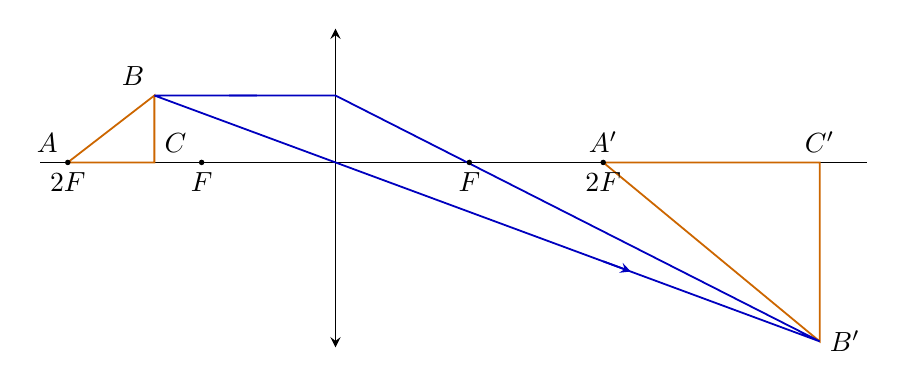
\begin{tikzpicture}[>=stealth,line width=.65pt]\draw(-3.75,0)--(6.75,0);\draw[<->](0,-2.35)--(0,1.7);\draw[orange!80!black](-3.4,0)--(-2.3,.85)--(-2.3,0)--cycle (3.4,0)--(6.15,-2.273)--(6.15,0)--cycle;\draw[blue!75!black](-2.3,.85)--(0,.85)--(6.15,-2.273) (-2.3,.85)--(6.15,-2.273);\draw[->,blue!75!black](-1.35,.85)--(-1,.85) (3.4,-1.256)--(3.75,-1.385);\foreach \x/\l in {-3.4/2F,-1.7/F,1.7/F,3.4/2F}{\fill (\x,0)circle(.035)node[below]{$\l$};}\node[above left]at(-3.4,0){$A$};\node[above left]at(-2.3,.85){$B$};\node[above right]at(-2.3,0){$C$};\node[above]at(3.4,0){$A^{\prime}$};\node[above]at(6.15,0){$C^{\prime}$};\node[right]at(6.15,-2.273){$B^{\prime}$};\end{tikzpicture}\end{center}


Изображение точки B удобно найти как пересечение луча, проходящего через центр линзы и луча, падающего на линзу параллельно главной оптической оси.
Изображение точки С находится в точности под изображением точки В. Положение изображения точки А легко определить из формулы тонкой линзы: 

\[\frac{1}{d} + \frac{1}{f} = \frac{1}{F}\]

Поскольку точка А находится в двойном фокусе, то $d=2F,$ а значит, и $f=2F,$ то есть изображение точки А также находится в двойном фокусе.
Наконец, легко понять, что изображение треугольника вновь будет треугольником. Действительно, если пропустить луч через сторону ВА, то после преломления на этом луче будут находиться изображения всех точек со стороны ВА, то есть гипотенуза прямоугольного треугольника перейдет в гипотенузу треугольника-изображения.

Определим фокусное расстояние

\[F= \frac{1}{D} = \frac{1}{2{,}5\,\text{дптр}} =0{,}4\,\text{м}.\]

Обозначим катет треугольника ABC через $h.$
Найдем расстояние от линзы до изображения точки С ($d=2F - h$):

\[f= \frac{dF}{d - F} = \frac{( 2 \cdot 40 \,\text{см} - 4\,\text{см} ) \cdot 40\,\text{см}}{2 \cdot 40 \,\text{см} - 4\,\text{см} - 40\,\text{см}} \approx 84{,}4\,\text{см}.\]

Горизонтальный катет равен 

\[a=f - 2F\approx 4{,}4\,\text{см}.\]

Из подобия треугольников для вертикального катета треугольника-изображения имеем

\[\frac{h}{b} = \frac{d}{f} \Longleftrightarrow b= \frac{hf}{2F - h} \approx 4{,}4 \,\text{см}.\]

Таким образом, площадь треугольника изображения равна: 

\[S' = \frac{1}{2} ab = \frac{1}{2} ( 4{,}4\,\text{см} ) ^2 \approx 10\,\text{см} ^2 .\]

Ответ: $10\,\text{см} ^2$

Примечание:
В решение можно было использовать тот факт, что треугольник-изображение также является равнобедренным. Это следует из того факта, что луч, проходящий через двойной фокус после преломления в линзе снова попадет в двойной фокус. Тем самым после преломления в линзе луч идет по тем же самым углом к главной оптической оси, что и до преломления в линзе. Поскольку в нашем случае этот угол равен $45 ^\circ,$ то равнобедренный треугольник снова получится равнобедренным.
}

% Source sdamgia-43830: https://phys-ege.sdamgia.ru/problem?id=43830
\BankTask{sdamgia-43830}{
\begin{center}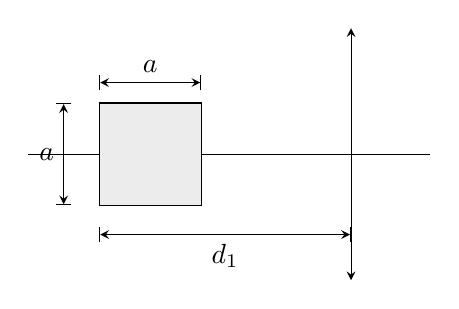
\begin{tikzpicture}[>=stealth]

\draw (-4.1,0)--(1,0);\draw[<->](0,-1.6)--(0,1.6);
\draw[fill=gray!15](-3.2,-.65)rectangle(-1.9,.65);
\draw[|<->|](-3.2,.91)--(-1.9,.91)node[midway,above]{$a$};
\draw[|<->|](-3.65,-.65)--(-3.65,.65)node[midway,left]{$a$};
\draw[|<->|](-3.2,-1.02)--(0,-1.02)node[midway,below]{$d_1$};
\end{tikzpicture}\end{center}
Квадрат со стороной a  =  $20\,\text{см}$ расположен в плоскости главной оптической оси тонкой собирающей линзы с оптической силой D  =  $2\,\text{дптр}$ так, что две его стороны параллельны плоскости линзы (см. рис.). Расстояние от дальней стороны квадрата до плоскости линзы $d_{1}$  =  $90\,\text{см}$. Определите площадь изображения квадрата в линзе. Сделайте рисунок, на котором постройте изображение квадрата в линзе, указав ход всех необходимых для построения лучей.
}{
\smallskip\noindent\textbf{Решение}\par
Обозначим вершины квадрата ABCD, тогда AB  =  AD  =  a.  
Для построения изображения квадрата проведём побочные оптические оси AO и BO, а также луч AB, параллельный главной оптической оси, который, преломившись, пройдёт через фокус линзы. В силу симметрии предмета относительно главной оптической оси его изображение также будет симметричным. В результате построений получим изображение квадрата ABCD в виде равнобедренной трапеции $A_{1}$$B_{1}$$C_{1}$$D_{1}$ (см. рис.).
\begin{center}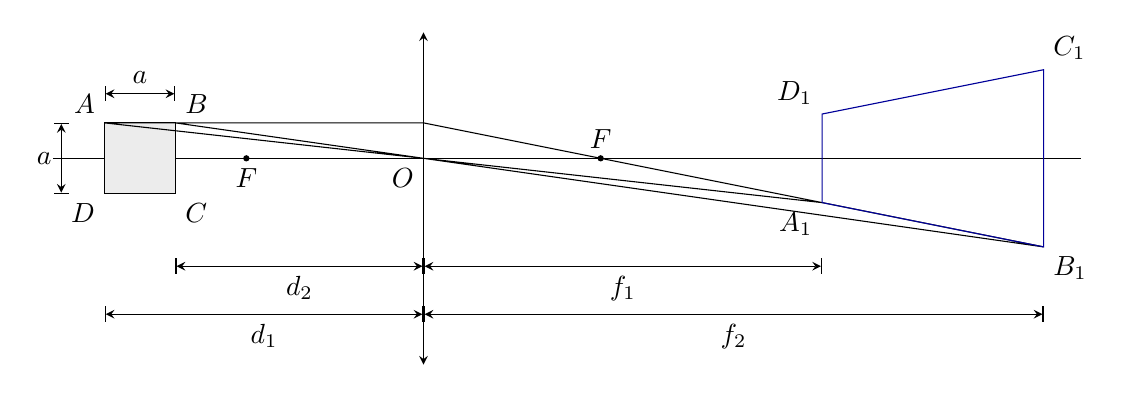
\begin{tikzpicture}[>=stealth]

\draw (-4.7,0)--(8.35,0);\draw[<->](0,-2.62)--(0,1.6);\node[below left] at(0,0){$O$};
\draw[fill=gray!15](-4.05,-.45)rectangle(-3.15,.45);
\node[above left]at(-4.05,.45){$A$};\node[above right]at(-3.15,.45){$B$};
\node[below right]at(-3.15,-.45){$C$};\node[below left]at(-4.05,-.45){$D$};
\fill (-2.25,0)circle(.04) node[below]{$F$} (2.25,0)circle(.04)node[above]{$F$};
\draw (-4.05,.45)--(0,.45)--(7.875,-1.125) (-4.05,.45)--(5.0625,-.5625) (-3.15,.45)--(7.875,-1.125);
\draw[blue!60!black] (5.0625,-.5625)--(7.875,-1.125)--(7.875,1.125)--(5.0625,.5625)--cycle;
\node[below left]at(5.0625,-.5625){$A_1$};\node[below right]at(7.875,-1.125){$B_1$};
\node[above right]at(7.875,1.125){$C_1$};\node[above left]at(5.0625,.5625){$D_1$};
\draw[|<->|](-4.05,.82)--(-3.15,.82)node[midway,above]{$a$};
\draw[|<->|](-4.6,-.45)--(-4.6,.45)node[midway,left]{$a$};
\draw[|<->|](-3.15,-1.37)--(0,-1.37)node[midway,below]{$d_2$};
\draw[|<->|](0,-1.37)--(5.0625,-1.37)node[midway,below]{$f_1$};
\draw[|<->|](-4.05,-1.98)--(0,-1.98)node[midway,below]{$d_1$};
\draw[|<->|](0,-1.98)--(7.875,-1.98)node[midway,below]{$f_2$};
\end{tikzpicture}\end{center}

Согласно формуле оптической силы линзы $F = \frac{1}{D} = \frac{1}{2} = 0{,}5 \,\text{м} = 50 \,\text{см}.$ Расстояние от линзы до квадрата равно $d_2 = d_1 - a = 90 - 20 = 70 \,\text{см}.$ По формуле тонкой линзы определим расстояния от линзы до оснований трапеции:

$\frac{1}{F} = \frac{1}{d_1} + \frac{1}{f_1} ,$
$\frac{1}{F} = \frac{1}{d_2} + \frac{1}{f_2} .$

 В итоге

$f_1 = \frac{Fd_1}{d_1 - F} = \frac{50 \cdot 90}{90 - 50} = 112{,}5 \,\text{см},$
$f_2 = \frac{Fd_2}{d_2 - F} = \frac{50 \cdot 70}{70 - 50} = 175 \,\text{см}.$

 Высота трапеции $h = f_2 - f_1 = 62{,}5 \,\text{см}.$
Используя формулу увеличения линзы для двух сторон квадрата, получим

$\frac{AD}{d_1} = \frac{A_1D_1}{f_1} ,$
$\frac{BC}{d_2} = \frac{B_1C_1}{f_2} .$

 Следовательно,

$A_1D_1 = \frac{f_1 \cdot AD}{d_1} = \frac{112{,}5 \cdot 20}{90} = 25 \,\text{см},$
$B_1C_1 = \frac{f_2 \cdot BC}{d_2} = \frac{175 \cdot 20}{70} = 50 \,\text{см}.$

Площадь изображения (трапеции) определяется формулой

\[S = \frac{A_1D_1 + B_1C_1}{2} \cdot h = \frac{25 + 50}{2} \cdot 62{,}5 \approx 2344 \,\text{см} ^2 .\]

Ответ: $S \approx 2344 \,\text{см} ^2 .$
}

\end{document}
